\section{Arquitectura}
Entenda-se por servidor como o conjunto de brokers interligados e base de dados. 
Os brokers são instâncias da mesma aplicação. Os brokers são idêntiocos à excepção dos endereços onde atendem ligações.
A ideia é ser indiferente o broker ao qual um cliente estabelece ligação uma vez que o comportamento é distribuído pelos restantes.
Por exemplo: dois clientes subscreveram o mesmo canal em brokers diferentes e um terceiro cliente envia uma mensagem para esse canal, então ambos os novos clientes recebem a mensagem.

\begin{figure}[H]
\centering
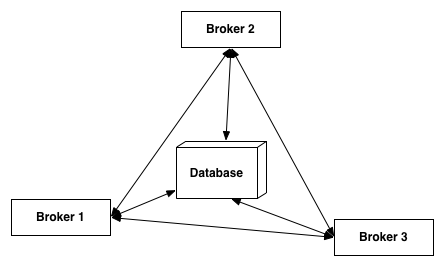
\includegraphics[width=0.65\textwidth]{brokers.png}
\caption{\textit{Visão simplista da arquitectura do servidor.}}
\label{fig:brokers-arq}
\end{figure}

A figura~\ref{fig:brokers-arq} apresenta um esquema simplista das ligações entre os diferentes componentes do servidor. O que se pode retirar do esquema é que os brokers estão ligados entre si e cada um está por sua vez ligado à base de dados.

A base de dados é responsável por armazenar as mensagens persistentes, manter uma sequência que forneça identificadores únicos aos clientes e manter um registo dos endereços dos servidores activos. Todas as restantes acções são da responsabilidade dos brokers. A ligação entre todos os brokers serve dois propósitos:

\begin{enumerate}
\item \textbf{Difundir mensagens}. As mensagens que um broker recebe são difundidas pelos restantes. Isto permite que vários clientes possam subscrever os mesmos canais quando estão ligados a brokers diferentes.
\item \textbf{Informar da actualização na lista de servidores}. Quando existe um novo broker online ou um dos brokers é identificado como inactivo o novo broker ou o broker que identificou o problema, respectivamente, actualizam a base de dados e enviam uma mensagem de actualização a todos os brokers.
\end{enumerate}
